% !TEX encoding = UTF-8
% !TEX TS-program = pdflatex
% !TEX root = ../Tesi.tex
% !TEX spellcheck = en-EN

%************************************************
\chapter{Aim of this Thesis}
\label{cap:aim}
%************************************************

In our study, we harnessed Artificial Neural Networks (\acs{ANNs}) in order to
reduce the number of \acs{DEM} test simulations required
to characterize bulk materials for large scale simulations. \\
As the following chapters will show, we divided this task in two sections:
\begin{enumerate}
  \item{identification of \acs{DEM} parameters, in part
  \ref{par:identification},}
  \item{applications, in part \ref{par:applications}.}
\end{enumerate}

\info{aim for regression from pca}

\section{Aim for Neural Network}
\label{sec:aimforneuralnetwork}

\acs{ANNs} have proven to be a versatile tool in analysing complex, non-linear
systems of multi-dimensional input streams (Vaferi et al. \cite{RefWorks:150}, Witten et
al. \cite{RefWorks:174} and Haykin \cite{RefWorks:158}).
In our case, we fed an \acs{ANN} with \acs{DEM} contact law parameters as input
and compared the output with the bulk behaviour 
predicted by a corresponding \acs{DEM} simulation. 
The difference between \acs{ANN} prediction and \acs{DEM} prediction was used to
train our specific \acs{ANN} with a backward-propagation algorithm. 
\begin{figure}[!htb]
\centering
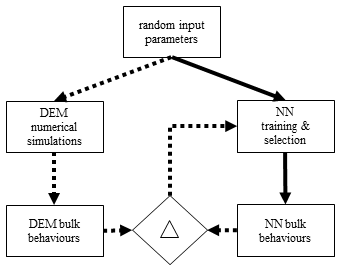
\includegraphics[width=.50\columnwidth]{images/127anntraining}
\caption[ANN training]{ANN training.}
\label{fig:127anntraining}
\end{figure}
After a training phase comprising a limited number of \acs{DEM} test simulations,
the \acs{ANN} could then be used as a stand-alone prediction tool for the bulk behaviour of a 
granular material in relation to \acs{DEM} contact law parameters, see Fig.
\ref{fig:127anntraining}. \\
In this study, we applied this parameter identification method to two different
granular bulk behaviours, namely the angle of repose (\acs{AoR}) test and the
Schulze shear cell (\acs{SCT}) test.
In both cases, we first trained a specific \acs{ANN} using a number of \acs{DEM} test
simulations before we identified valid sets of \acs{DEM} contact law parameters by
comparing the stand-alone \acs{ANN} predictions with corresponding bulk experiments. 
For both cases we obtained valid sets of contact law parameters, 
which we then compared to formulate a reliable contact law for a given
granular material.
We further showed that the same \acs{ANN} could be used to characterize different
granular materials, which have the same particle behaviour and could modelled with the same contact
law.

\begin{figure}[!htb] 
\centering 
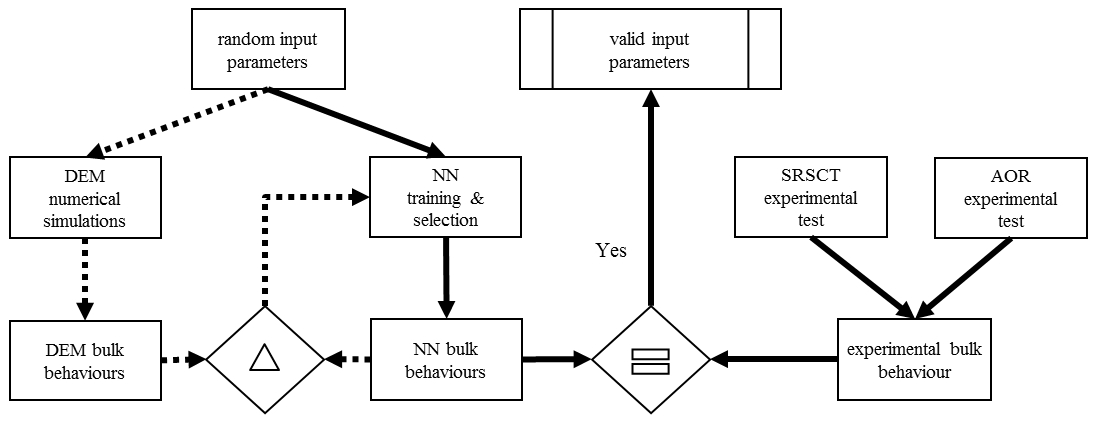
\includegraphics[width=.96\textwidth]{images/019methodology} 
\caption[Method]{Method. In the training phase (dashed lines)
$DEM$ simulations are performed
with random initial input parameters.
The behaviours obtained are used to train the
Artificial Neural Networks ($ANNs$) in a loop that continues until the
difference between the outputs of each $ANN$ and its simulations is below the
limit ($\Delta$).
In the parameters identification phase (solid
lines) we identify valid input parameters by comparing (\textbf{=}) $ANNs$ and
experimental behaviours.}
\label{fig:019methodology} 
\end{figure}


\subsection{Applicability and scope}
\label{subsec:applicability}

%************************************************
\begin{figure}[!htb] 
\centering 
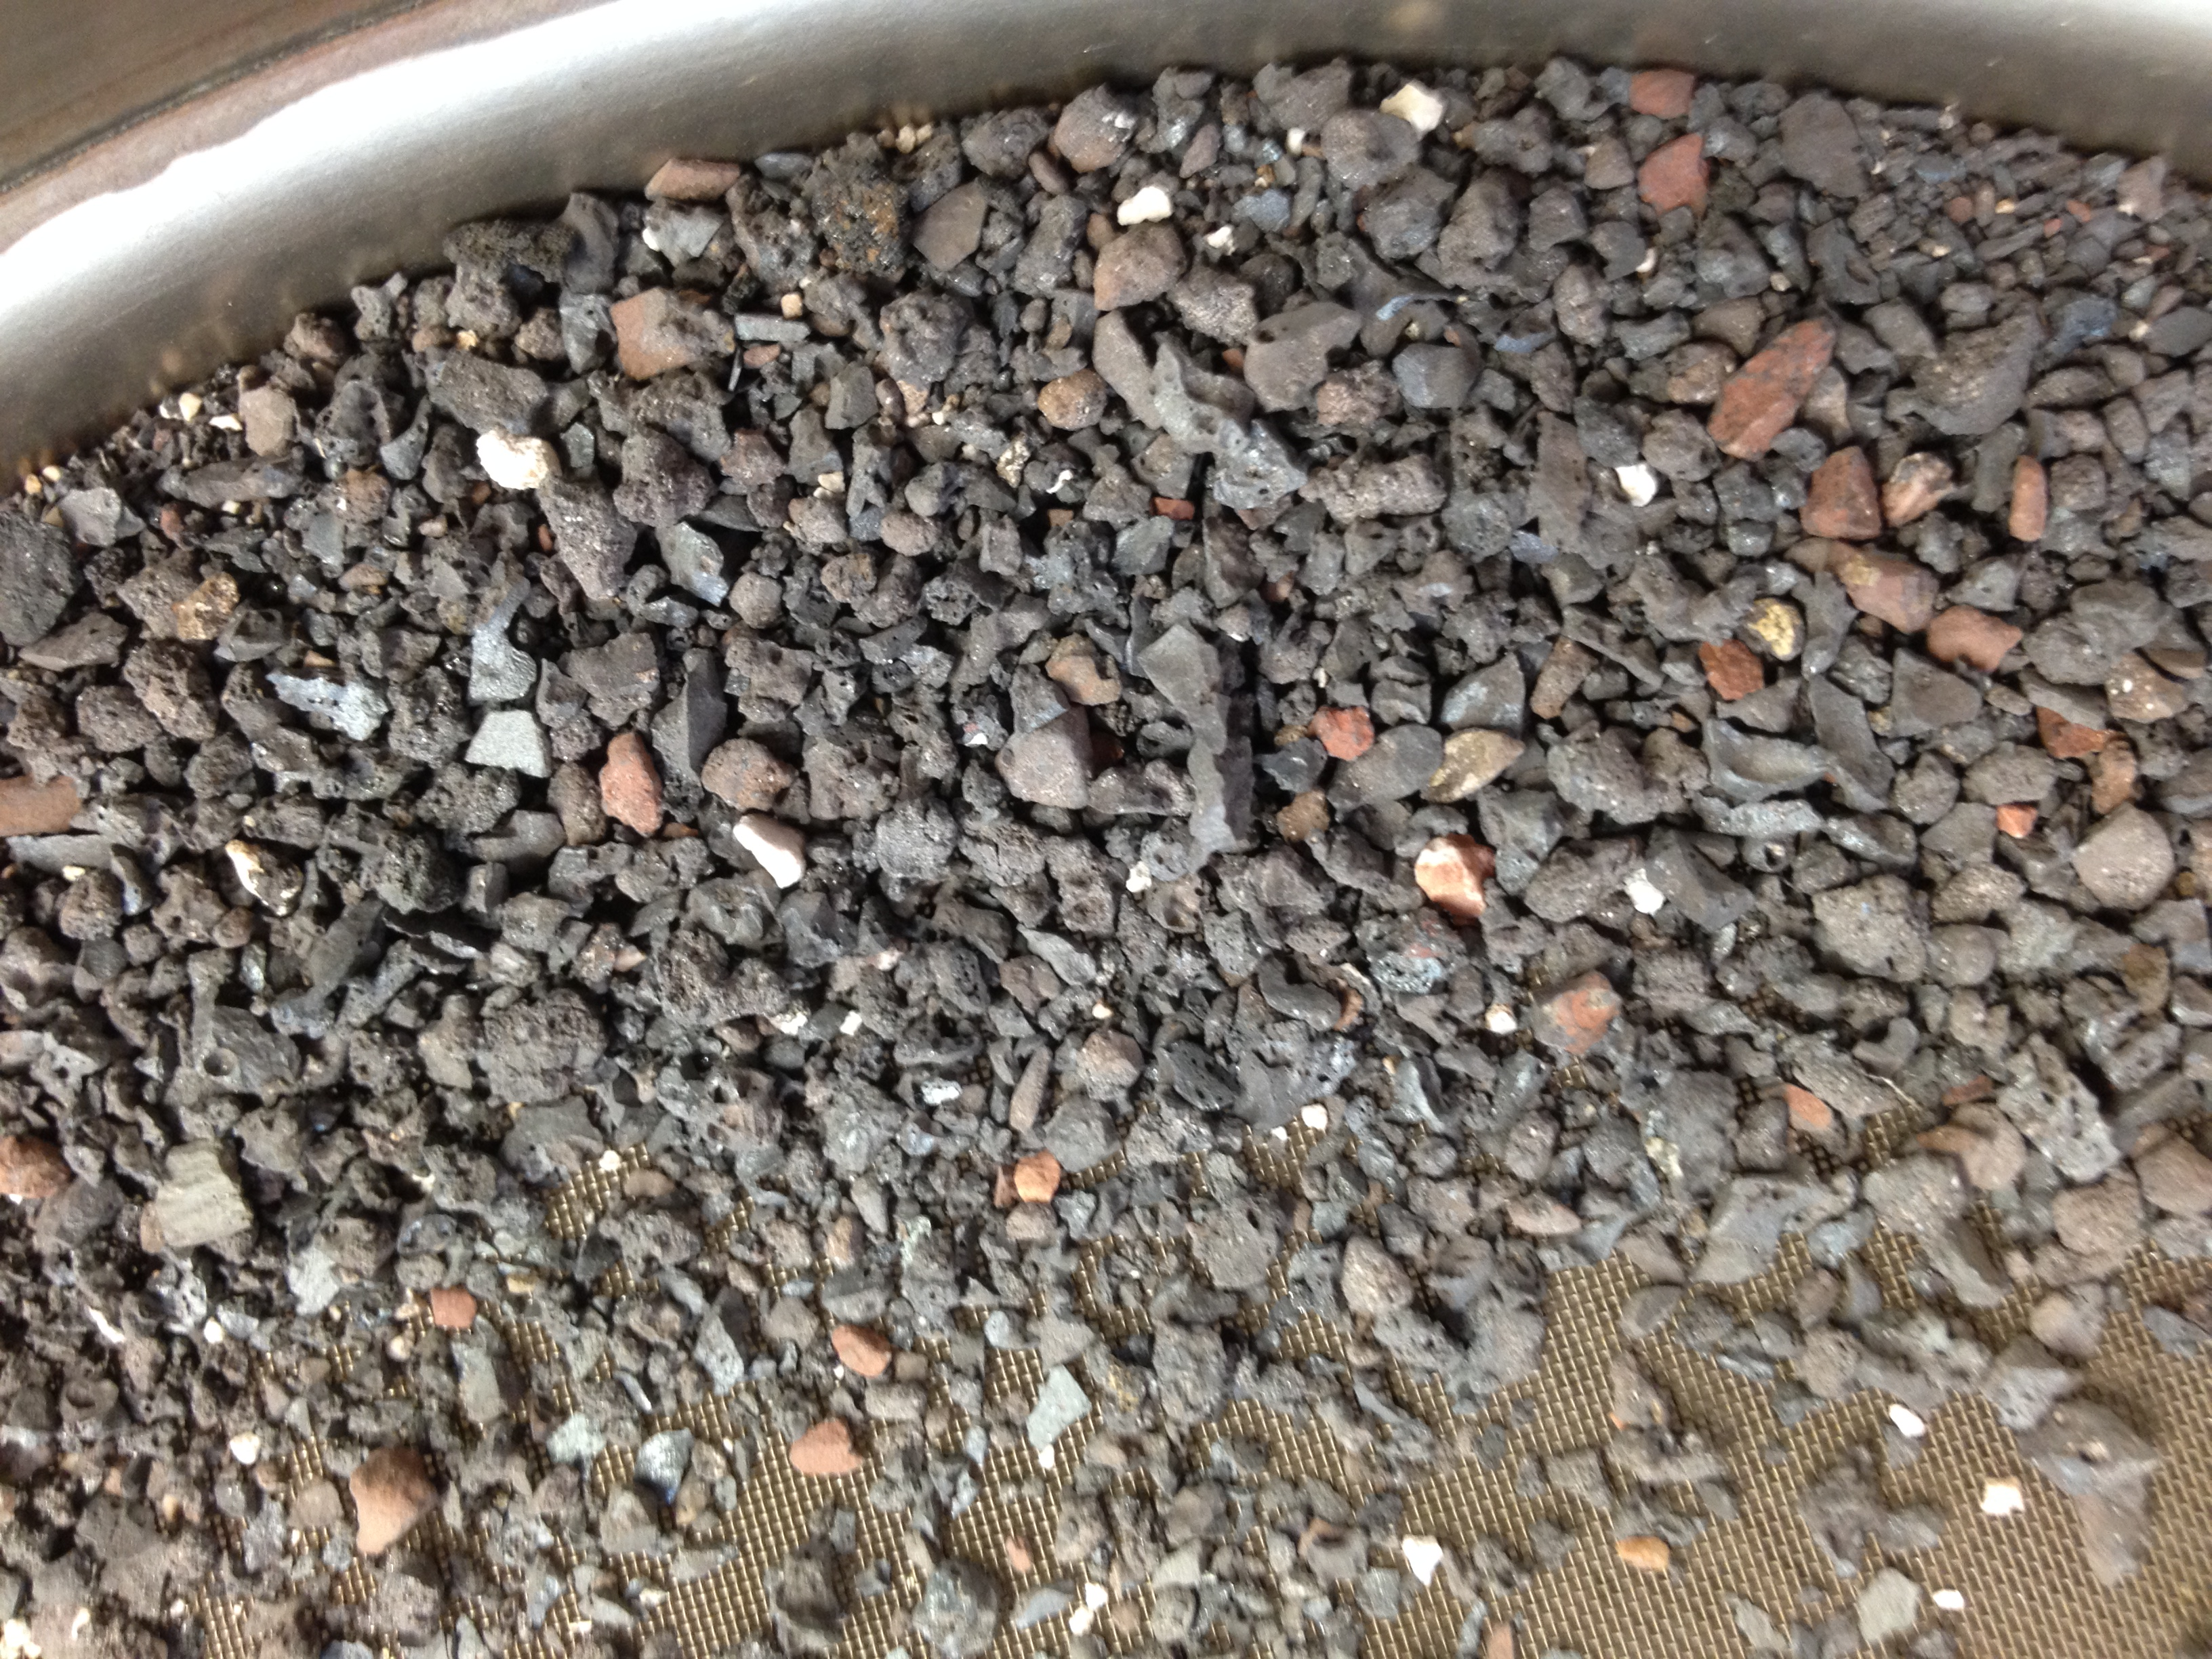
\includegraphics[width=.96\textwidth]{104material} 
\caption[Sinter ore fine]{Sinter ore fine analysed.}
\label{fig:104material} 
\end{figure}

%************************************************

The materials used for this work were sinter fine, see Fig.
\ref{fig:104material}, 
\wrong{add photos of all materials}
. Its particles had a mean radius of 0.73 mm and were
cohesionless, see Chapter \ref{cap:experimentalcharacterization}.
Their amounts of open and closed pores are not negligible (see
\citet{RefWorks:191}), 
and thus the use of an Archimedean procedure to determine the correct particle density by direct measurement
was not applicable.
Possibly, a tomography for each particle would lead to the particle density
(e.g., \citet{RefWorks:77}), but this analysis was infeasible: 
the necessary time for the the amount of material
analysed was unreasonable. 
Further, a three-dimensional scan of each particle would have surely physically
identified our particles, and made us able to confront them with other studies. 
The high shape dispersity made also this analysis impossible. 
We followed a different procedure, see Chapter \ref{cap:anntraining}.\\
To avoid the macroscopic plastic deformations analysed by Harthong et al. \cite{RefWorks:183} 
we checked for each simulation for its total duration that the packing density was 
lower than a defined limit. 
This threshold (0.671) was given by the packing density of the close random packing with the 
same size distribution, as suggested and with the software provided by Baranau, Tallarek 
et al. \cite{RefWorks:182, RefWorks:185}.
The experimental characterization was performed at environmental temperature and thus 
temperature was not considered in the numerical simulations. Chemical reactions and aging 
were also not part of the scope of this work.
Further, due to the limited number of experiments realized, a restricted number
of flow regimes were tested, and only one size distribution was considered. 
The authors are confident that these two limitations have not compromised the validity of the method. 
Rather, further investigations on these two aspects could again demonstrate its effectiveness. 
Notably, we chose an elastic model to picture the particle behaviour. If we try
to identify parameters for an elastic contact model in a system of non-elastic particles, this $ANN$ approach will fail. 
So choosing appropriate contact models is an essential pre-requisite for contact 
parameter identification by means of $ANN$. 
Moreover, $ANNs$ can give indications about the correctness of the chosen model, 
see Chapter \ref{cap:anntraining}.